


\section{Experiment}

\begin{figure*}
  \centering
  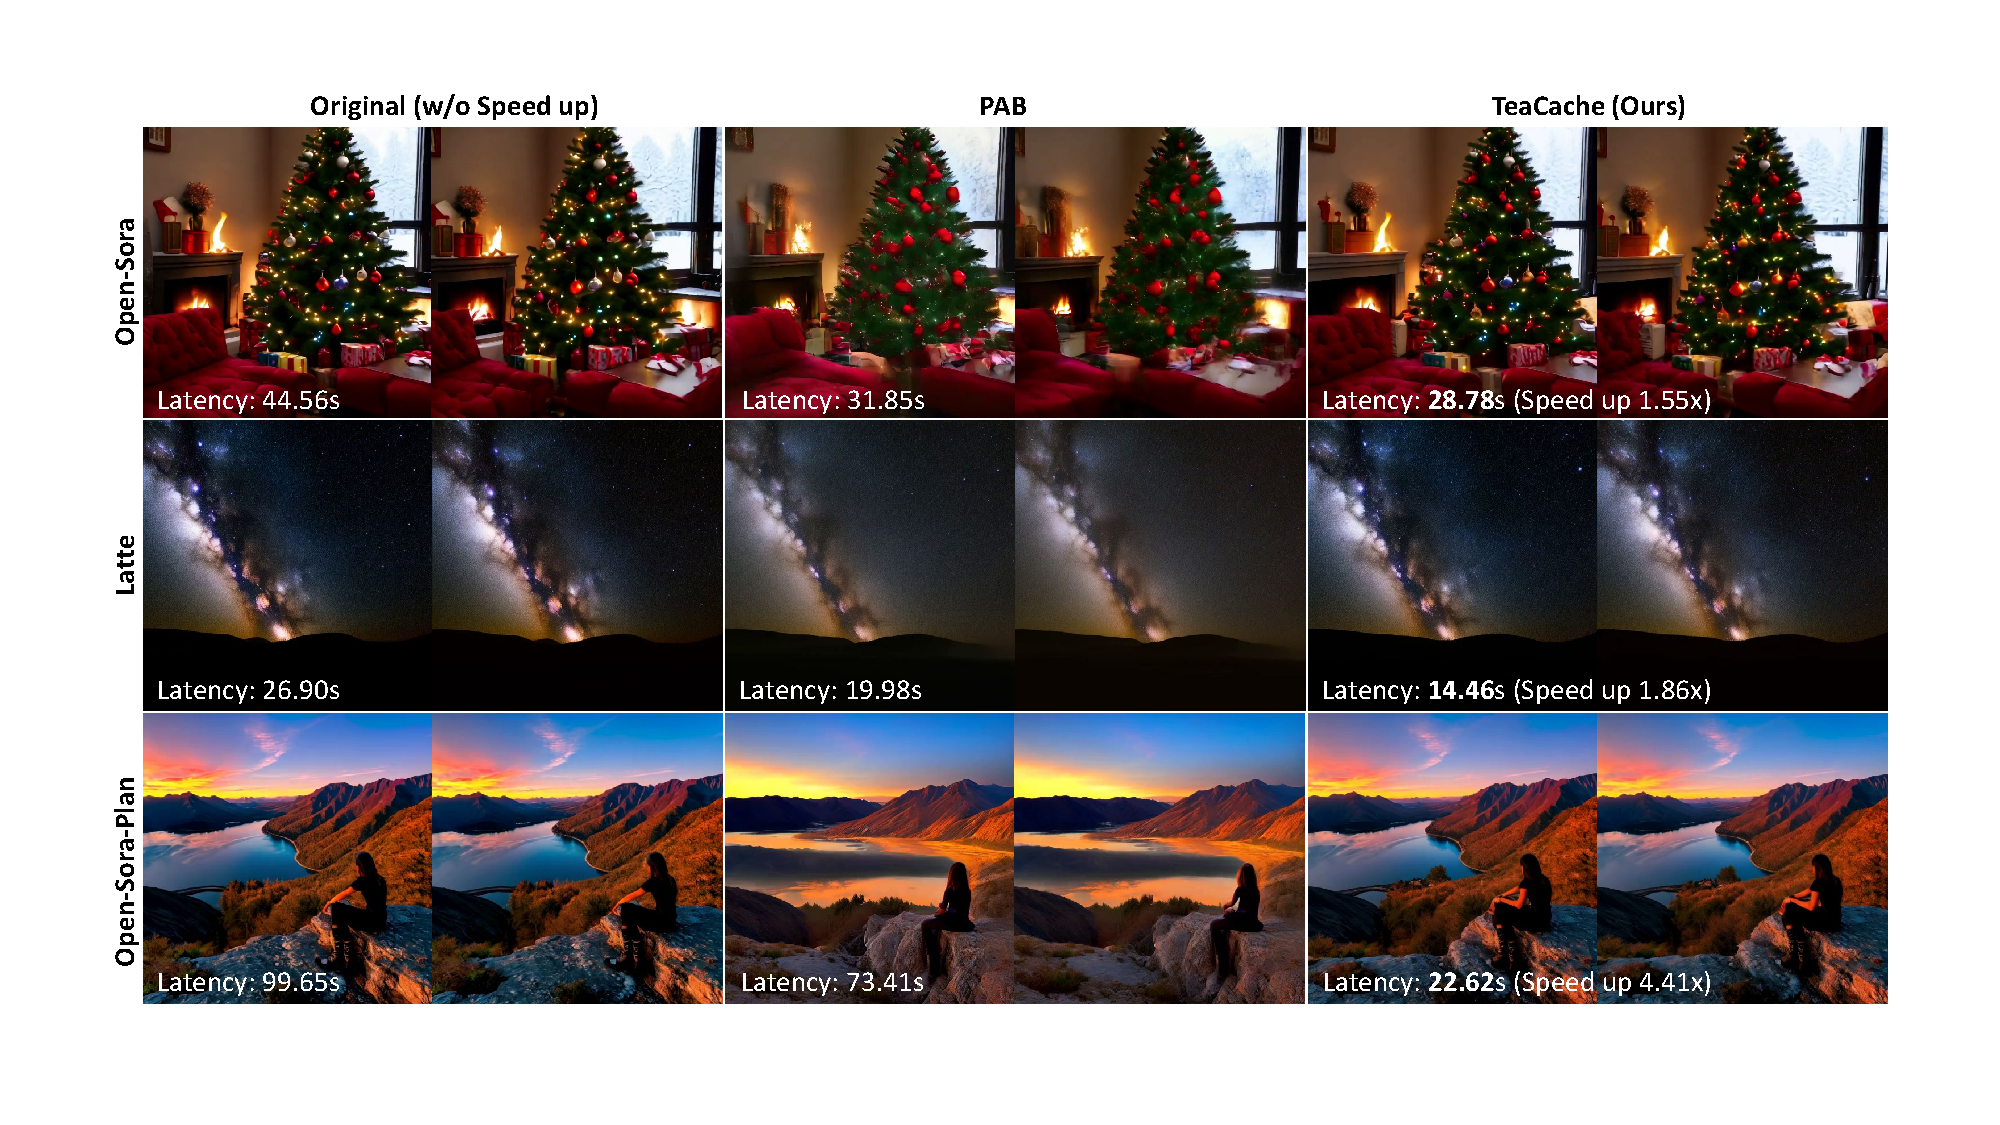
\includegraphics[width=0.98\linewidth]{figs/tisser.pdf}
  \caption{
  Comparison of visual quality and efficiency (denoted by latency) with the competing method. TeaCache outperforms PAB~\cite{zhao2024real} in both visual quality and efficiency. Latency is evaluated on a single A800 GPU. Video generation specifications: Open-Sora~\cite{Open-Sora} (51 frames, 480p), Latte~\cite{ma2024latte} (16 frames, 512$\times$512), Open-Sora-Plan~\cite{Open-Sora-Plan} (65 frames , 512$\times$512). Best-viewed with zoom-in.
  }
  \label{fig:show}
\end{figure*}



\subsection{Settings}
\textbf{Base Models and Compared Methods.} To demonstrate the effectiveness of our method, we apply our acceleration technique to various video, such as Open-Sora 1.2 ~\cite{Open-Sora}, Open-Sora-Plan~\cite{Open-Sora-Plan} and Latte~\cite{ma2024latte}. We compare our base models with recent efficient video synthesis techniques, including PAB~\cite{zhao2024real}, T-GATE~\cite{zhang2024cross} and $\Delta$-DiT~\cite{chen2024delta}, to highlight the advantages of our approach. Notably, $\Delta$-DiT and T-GATE are originally designed as an acceleration method for image synthesis; PAB adapted them for video synthesis to facilitate comparison. 

\textbf{Evaluation Metrics and Datasets.} To assess the performance of video synthesis acceleration methods, we focus on two primary aspects: inference efficiency and visual quality. For evaluating inference efficiency, we use Floating Point Operations (FLOPs) and inference latency as metrics. For visual quality evaluation, we employ VBench~\cite{huang2024vbench}, LPIPS~\cite{zhang2018unreasonable}, PSNR, and SSIM. VBench serves as a comprehensive benchmark suite for video generative models, aligning well with human perceptions and offering valuable insights from multiple perspectives. LPIPS, PSNR, and SSIM evaluate the similarity between videos produced by the accelerated sampling method and the original model. PSNR assesses pixel-level fidelity, LPIPS measures perceptual consistency, and SSIM evaluates structural similarity. Generally, higher similarity scores imply better fidelity and visual quality. The details of evaluation metrics are presented in Appendix.

\textbf{Implementation Detail} All experiments are carried out on the NVIDIA A800 80GB GPUs with Pytorch. We enable FlashAttention~\cite{dao2022flashattention} by default for all experiments.  To obtain robust polynomial fitting, we sample 70 texts from T2V-CompBench~\cite{sun2024t2v} to generate videos, assessing seven desired attributes of generated videos. 10 prompts are sampled for each attributes.
$\delta$ is 0.1 for TeaCache-slow and 0.2 for TeaCache-fast.


\begin{figure*}
    \centering
    \begin{minipage}{\textwidth}
    \centering
    \begin{subfigure}{0.24\textwidth}
        \centering
        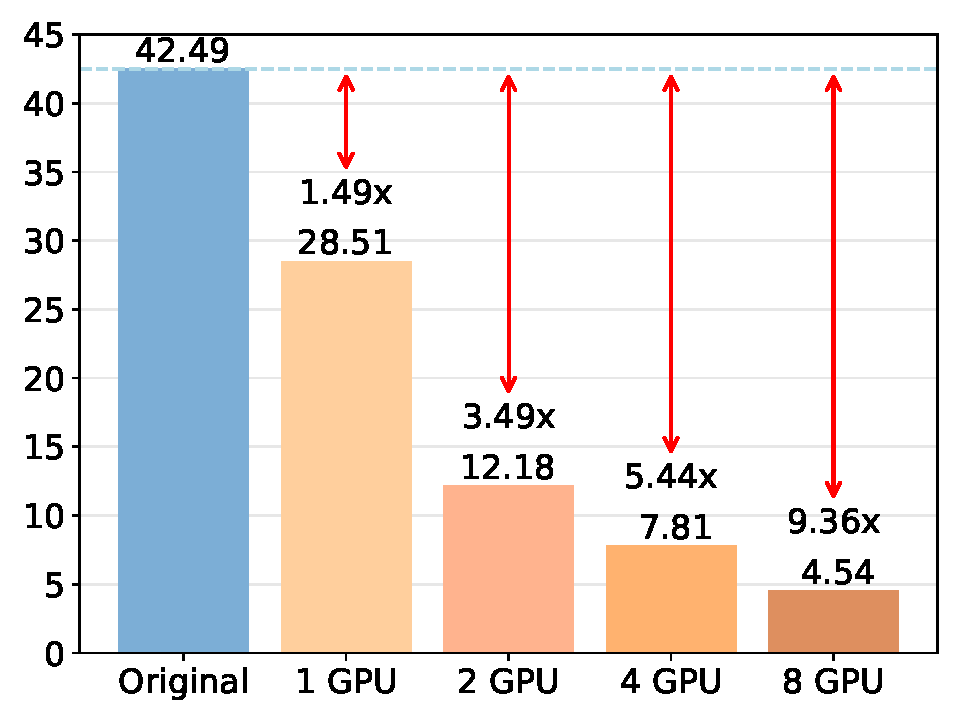
\includegraphics[width=\textwidth]{figs/480_48.pdf} 
        \caption{480P, 48 frames}
    \end{subfigure}
    \hfill
    \begin{subfigure}{0.24\textwidth}
        \centering
        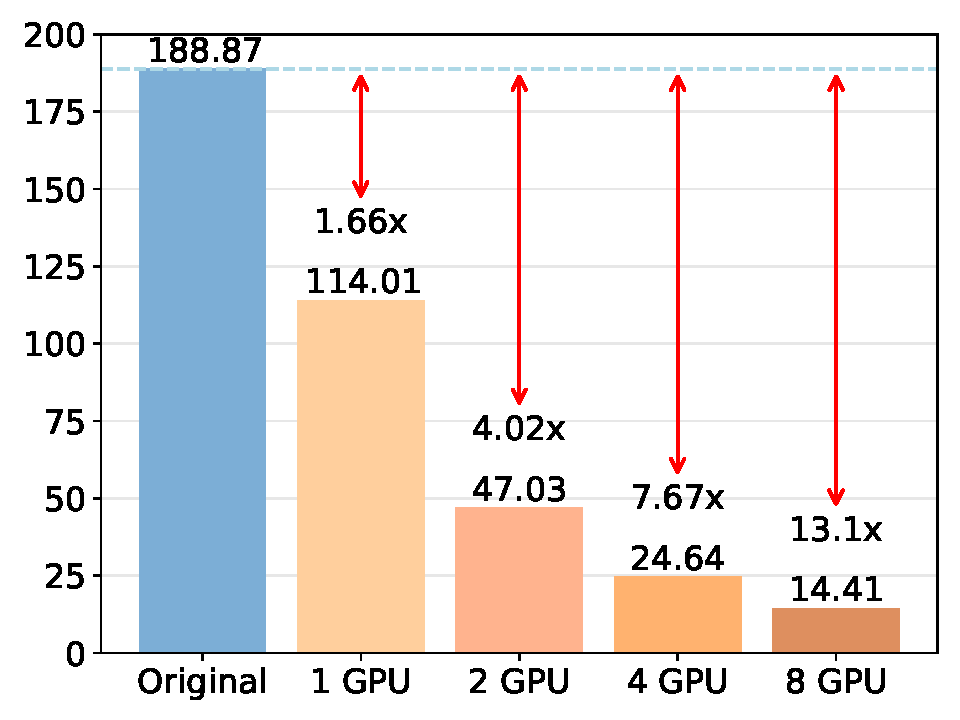
\includegraphics[width=\textwidth]{figs/480_192.pdf} 
        \caption{480P, 192 frames}
    \end{subfigure}
    \hfill
    \begin{subfigure}{0.24\textwidth}
        \centering
        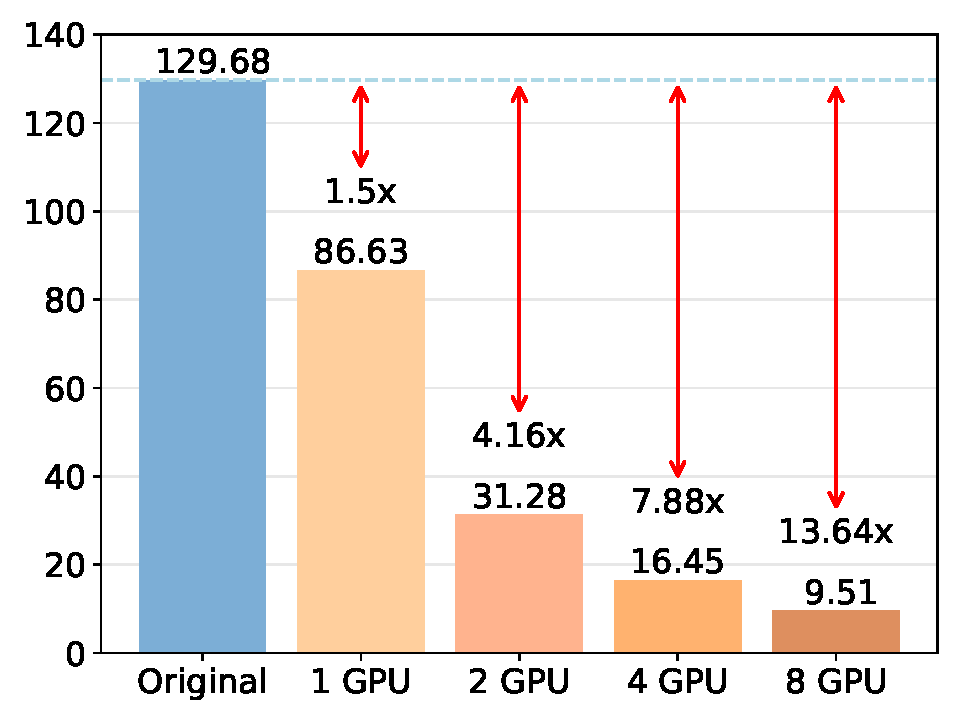
\includegraphics[width=\textwidth]{figs/360_240.pdf}
        \caption{360P, 240 frames}
    \end{subfigure}
    \hfill
    \begin{subfigure}{0.24\textwidth}
        \centering
        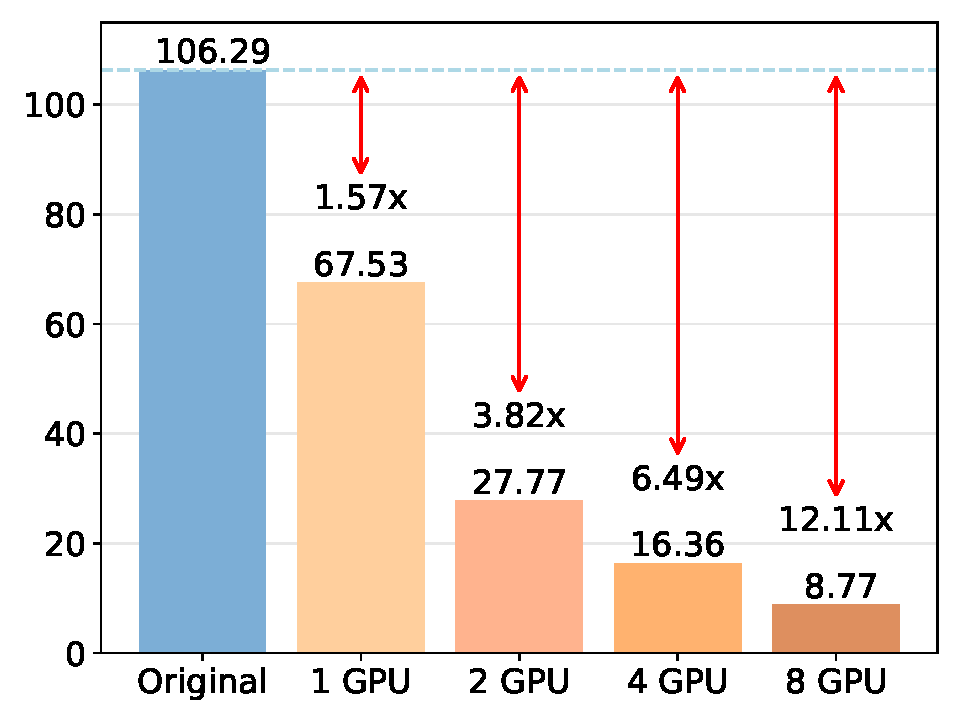
\includegraphics[width=\textwidth]{figs/720_48.pdf}
        \caption{720P, 48 frames}
    \end{subfigure}

    \end{minipage}

    \caption{Inference efficiency and visual quality of TeaCache at different video lengths and resolutions.}
    \label{fig:multi resolution}
\end{figure*}



\subsection{Main Results}

\textbf{Quantitative Comparison.} Tab.~\ref{tab: main} presents a quantitative evaluation of efficiency and visual quality using the VBench benchmark ~\cite{huang2024vbench}. We examine two variants of TeaCache: a slow variant and a fast variant with greater speedup. Compared to other training-free acceleration methods, TeaCache consistently achieves superior efficiency and better visual quality across different base models, sampling schedulers, video resolutions, and lengths. In evaluating the Latte~\cite{ma2024latte} baseline, the TeaCache-slow model demonstrates superior performance across all visual quality metrics, achieving a 1.86× speedup compared to PAB~\cite{zhao2024real}, which provides a 1.34× speedup. TeaCache-fast achieves the highest acceleration at 3.28×, albeit with a slight reduction in visual quality. With the OpenSora~\cite{Open-Sora} baseline, we obtain the optimal speedup of 2.25× as compared to the previous 1.40×, and the highest overall quality with a speedup of 1.55×. Additionally, using Open-Sora-Plan~\cite{Open-Sora-Plan}, TeaCache achieves the highest speedup of 6.83×, surpassing the previously best 1.49× offered by PAB, while also delivering the highest quality at a speedup of 4.41×.


\textbf{Visualization.} Fig.~\ref{fig:show} compares the videos generated by TeaCache against those by the original model and  PAB. The results demonstrate that TeaCache outperforms PAB in visual quality with lower latency. More visual results can be found in the Appendix.

\subsection{Ablation Studies}




\textbf{Scaling to multiple GPUs.} Aligned with previous research employing Dynamic Sequence Parallelism (DSP)~\cite{zhao2024real} for supporting high-resolution long-video generation across multiple GPUs, we assess the performance of TeaCache in these scenarios.  
The results of this study are presented in Tab.~\ref{tab: multiple GPU}. We utilize Open-Sora~\cite{Open-Sora} (480p - 192 frames at 30 timesteps) and Open-Sora-Plan~\cite{Open-Sora-Plan} (512×512 - 221 frames at 150 timesteps) as baselines and compare them against the prior method PAB~\cite{zhao2024real} regarding latency measurements on A800 GPUs. As the number of GPUs increases, TeaCache consistently improves inference speed across various base models and outperforms PAB. 


\textbf{Performance at different Length and Resolution.} To assess the effectiveness of our method in accelerating sampling for videos with varying sizes, we perform tests across different video lengths and resolutions. The results, presented in Fig.~\ref{fig:multi resolution}, demonstrate that our method sustains consistent acceleration performance, even with increases in video resolution and frame count. This consistency highlights the method's potential to accelerate sampling processes for longer and higher-resolution videos, meeting practical demands.

\textbf{Quality-Efficiency trade-off.} In Fig.~\ref{fig:shot}, we compare the quality-latency trade-off of TeaCache with PAB~\cite{zhao2024real}. Our analysis reveals that TeaCache achieves significantly higher reduction rates, indicated by lower absolute latency, compared to PAB. Additionally, across a wide range of latency configurations, TeaCache consistently outperforms PAB on all quality metrics. This is particularly evident in the reference-free metric VBench score~\cite{huang2024vbench}, which aligns more closely with human preferences. Although there is a decline in reference-based scores such as PSNR and SSIM at extreme reduction rates, qualitative results suggest that the outputs remain satisfactory, despite not perfectly matching the reference.

\textbf{Choice of Indicator.} When determining the caching schedule, we evaluate various indicators to estimate the differences in model outputs across consecutive timesteps. These indicators include timestep embedding and timestep embedding-modulated noisy input. As illustrated in Fig.~\ref{fig:difference}, the timestep embedding-modulated noisy input demonstrates a stronger correlation with model output compared to the timestep embedding, particularly in the OpenSora. Moreover, the selection of timesteps by the timestep embedding-modulated noisy input adapts dynamically to different prompts, whereas the timestep embedding selects the same timesteps for all prompts. This observation is validated by the results presented in Tab.~\ref{tab:indicator}, where the timestep embedding-modulated noisy input consistently surpasses the timestep embedding across various models, especially in OpenSora.

\textbf{Effect of Rescaling.} Tab.\ref{tab:fitting} illustrates the impact of rescaling. A first-order polynomial fitting outperforms the original data by 0.24\% under Vbench score metric, as well as in LPIPS, SSIM, and PSNR metrics. Performance gains tend to saturate with a fourth-order polynomial fitting.




\begin{table}[]
\scriptsize
\centering
    \caption{Ablation study of caching indicator. `Timestep': timestep embedding. `Input': timestep embedding-modulated noisy input.}
    % `Input' consistently outperforms `Timestep' with several models.}
    \label{tab:indicator}
\begin{tabular}{c|cccc}
\toprule
\textbf{Indicator}             &\textbf{VBench $\uparrow$} & \textbf{LPIPS $\downarrow$} & \textbf{SSIM $\uparrow$} & \textbf{PSNR $\uparrow$} \\
\hline
\rowcolor[gray]{0.9}OpenSora              & 79.22\%          &  -         &  -         &  -    \\
Timestep    & 77.01\% & 0.3425          & 0.6934          & 15.86     \\
Input & \textbf{78.21}\%  & \textbf{0.2549}  & \textbf{0.7457}  & \textbf{19.05}    \\
\hline
\rowcolor[gray]{0.9}Latte              & 77.40\%          &  -         &  -         &  -    \\
Timestep    &77.05\%  & 0.2653          &   0.7073        &  19.76    \\
Input & \textbf{77.17}\% & \textbf{0.2558} & \textbf{0.7164} & \textbf{20.00}  \\
\bottomrule
\end{tabular}
\end{table}

\vspace{-0.5em}



\begin{table}[]
\scriptsize
\centering
    \caption{Ablation study of polynomial fitting. Rescaling with polynomial fitting outperforms original data. Higher-order fitting obtains better performance and saturates in 4-order fitting. }
    \label{tab:fitting}
\begin{tabular}{c|cccc}
\toprule
\textbf{Order}             &\textbf{VBench $\uparrow$} & \textbf{LPIPS $\downarrow$} & \textbf{SSIM $\uparrow$} & \textbf{PSNR $\uparrow$} \\
\hline
\rowcolor[gray]{0.9}OpenSora              & 79.22\%          &  -         &  -         &  -    \\
Original    & 78.21\%  & 0.2549  & 0.7457  & 19.05     \\
1-order &78.45\%  &0.2517  &\textbf{0.7478}  &19.10   \\
2-order &78.48\%  &0.2513  &0.7477  &19.09   \\
4-order &\textbf{78.48}\% & \textbf{0.2511} & 0.7477 & \textbf{19.10}   \\
\bottomrule
\end{tabular}
\end{table}

\begin{table}[]
\scriptsize
\centering
\caption{Inference efficiency and visual quality when scaling to multiple GPUs with Dynamic Sequence Parallelism (DSP).}
\label{tab: multiple GPU}
\scalebox{0.92}{
\begin{tabular}{l|c|c|c|c}
\toprule
\textbf{Method} & 1 × A800 & 2 × A800 & 4 × A800 & 8 × A800 \\ 
\hline
\multicolumn{5}{c}{\textbf{Open-Sora (192 frames, 480P)}} \\ \hline
Baseline &  188.87(1×) &  72.86(2.59×) &  39.26(4.81×) &  22.18(8.52×) \\ \hline
PAB &  142.23(1.33×) &  53.74(3.51×) &  29.19(6.47×) &  16.88(11.19×) \\ \hline
\rowcolor{gray!30} TeaCache &  114.01(1.66×) &  47.03(4.02×) &  24.64(7.67×) &  14.41(13.10×) \\ \hline
\multicolumn{5}{c}{\textbf{Open-Sora-Plan (221 frames, 512×512)}} \\ \hline
Baseline &  324.41(1×) &  166.94(1.94×) &  88.18(3.68×) &  47.79(6.79×) \\ \hline
PAB &  207.70(1.56×) &  110.06(2.95×) &  58.07(5.59×) &  31.92(10.16×) \\ \hline
\rowcolor{gray!30} TeaCache &  48.22(6.73×) &  26.99(12.02×) &  15.91(20.39×) & 10.13 (32.02×) \\ 
\bottomrule
\end{tabular}
}
\end{table}
